% We are thrilled to announce the launch of the groundbreaking ByteBoost Cybertraining Program. ByteBoost is driven by the imperative to enhance researchers' proficiency and productivity when navigating cutting-edge, specialized computing technologies. We hope to empower researchers to make the best computing choices in the ever-changing landscape of computational technology. This initiative will focus on supporting researchers using the technologies of three NSF computing testbeds - Ookami, Neocortex and ACES.

% Program Objectives:
% Facilitate Seamless Research: Elevate the ease and productivity of researchers working with cutting-edge computing technology.
% Community Growth: Foster a well-informed community of computational researchers adept at handling the newest technologies and porting applications.
% Optimal Testbed Usage: Ensure the proper and efficient utilization of testbeds, a critical component in the recent surge of data-enabled science and engineering.
% Target Audience:
% Early career-researchers (graduate students, postdoctoral associates, and Assistant Professors) from all fields of computationally inclined research

% Submission Guidelines
% Submission must include the following
% CV (1 page) including the applicant's previous computing experiences, skills, and field of science
% Abstract (1 page) - Prospective participants are required to submit an abstract outlining the specific topic they intend to explore as a fundamental part of their application for consideration in this call for participation.
\noindent
\textit{\textbf{Foundations for Agent-based Evolution Simulation on Emerging HPC Accelerators.}}
\hfill
{\scriptsize M.A. Moreno, \texttt{morenoma@umich.edu}}

\section{Introduction}
Evolutionary processes underlie key questions in public health, medicine, and natural resources management.
In conjunction with benchtop experiments and observational studies, \textbf{mathematical and computational models play a key role in understanding evolutionary processes} underpinning critical problems like epidemiology, antibiotic resistance, cancer biology, and conservation biology.
Emerging High-Performance Computing (HPC) hardware like the Cerebras Wafer-Scale Engine (WSE) will \textbf{enable detailed modeling of cross-scale evolutionary phenomena}, such as major transitions in individuality (e.g., evolution of multicellularity) and evo-epidemiological tradeoffs between pathogens' within-host dynamics and between-host transmissibility \cite{goldsby2020major,schreiber2021evolutionary}.

\section{Objectives}

The proposed workshop project will create foundational \textbf{algorithms and kernel implementations in Cerebras Software Language (CSL)} necessary to harness emerging HPC hardware accelerators for agent-based evolution simulation.
Developed simulation will investigate how \textbf{population structure and rare mutational events influence selective sweep frequency} within very large populations.
Among other application areas, sweep dynamics are pivotal in epidemiology to understanding how new disease strains emerge and establish \cite{markov2023evolution}.

\section{Methods}

To succeed as a tool for scientific research, simulation must be sufficiently observable.
In the case of evolutionary simulation, \textbf{phylogenetic history} (i.e., ancestry trees) \textbf{is key to assessing the mode and tempo of evolution}.

\begin{wrapfigure}{R}{2in}
% \begin{minipage}{3in}
\vspace{-3ex}
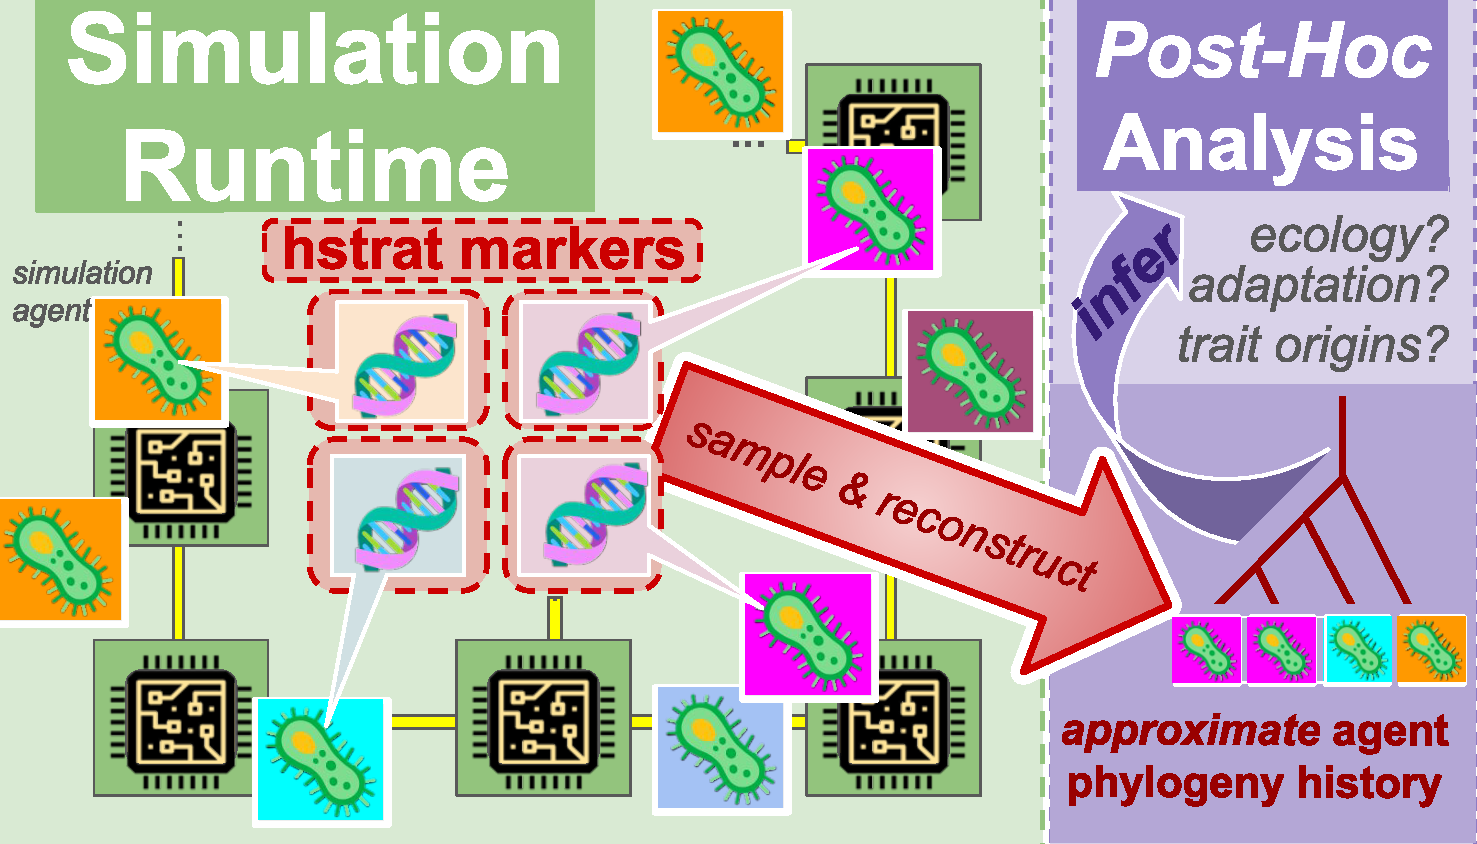
\includegraphics[width=2in]{img/runtime-posthoc-schematic.pdf}
% \end{minipage}%
% \begin{minipage}{2in}
\vspace{-5ex}
\caption{\footnotesize
Evolution simulation with reconstruction-based lineage analysis.}
\label{fig:runtime-posthoc-schematic}
\vspace{-2ex}
% \end{minipage}
\end{wrapfigure}


Proposed work builds on new \textbf{\textit{hereditary stratigraphy} (HStrat) methods} designed to enable \textbf{extraction of evolutionary history from decentralized, many-processor simulations} \cite{moreno2022hstrat}.
These methods mark population members with a special annotation akin to noncoding DNA, inherited by each consecutive generation.
After simulation ends, HStrat markers facilitate fast and accurate \textbf{reconstruction of phylogenetic history}.
This procedure (Fig. \ref{fig:runtime-posthoc-schematic}) analogizes use of DNA sequence data to infer phylogenies of natural systems.
Unlike direct lineage tracking, HStrat methods scale gracefully to long-running multiprocess simulation \cite{moreno2024analysis}.
Markers can be as small as 96 bits.

Simulation will use an \textbf{island-model algorithm} to support very large population sizes.
This approach instantiates separate agent subpopulations per processing element (PE), with agents occasionally migrated between subpopulations.
Rates of agent migration and the pattern of connectivity between islands determines global population structure.

A simple agent model suffices for proposed work, with agent traits abstracted to a floating-point ``fitness'' value encoded directly in agent genomes.
Fitness landscape properties can be tuned through choice of mutation operator.
For instance, increased probability for large fitness losses would simulate a rugged landscape.

\section{Proposed Work}

Capstone work will build on recent \textbf{prototype implementation} of HStrat-enabled island model evolutionary simulation in CSL using the v1.0.0 Cerebras SDK, available via GitHub at \texttt{\href{https://hopth.ru/cl}{hopth.ru/cl}}.
However, several engineering problems suited to workshop capstone scope remain to be solved:
\begin{enumerate}[leftmargin=*]
\item \textbf{Agent migration between distant processing elements}.
Implementation of long-distance migration will enable manipulation of population structure via changes to island connectivity.
Possible strategies include stochastic forwarding or more structured wavelet routing schemes.
Ideally, implementation will take advantage of WSE routing intrinsics to avoid consuming PE cycles by explicitly forwarding at each PE hop.

\item \textbf{On-the-fly device-to-host agent sampling.}
Full understanding of evolutionary history requires access to lineage intermediates (i.e., a ``fossil record'').
This problem concerns how to stream a rolling, random subsample of agent genomes to the wafer periphery then back to the host machine.
Bandwidth use will need to be balanced against between-PE agent migration.
As a simplification, sampling could be restricted to only consider wafer-edge PEs.
\end{enumerate}

\section{Outcomes}

First, agent migration and sampling will be \textbf{validated for correctness and profiled for performance}.
Apropos the former, we will test using genomes annotated with the ID of their originating PE.
The latter will assess induced effects on generations elapsed per unit walltime as well as update rate across PE counts (weak scaling).

To \textbf{investigate selective sweep dynamics}, we will use HStrat to compare the most recent common ancestor (MRCA) times of populations evolved with weak vs. strong population structure (viz. migration rate) and with vs. without fat-tailed mutational effect size.
We will test effect interactions with population scale by varying PE count.
